\section{Monetary Policy}
\label{sec:mp}

\textbf{OCTA} is the primary payment instrument and the currency used to pay for the services provided by OctaSpace, as well as rewards to node owners and dividend payments for OCTA holders.

In order to maintain stable inflation levels, OctaSpace implements a finite monetary policy.

The policy consists of a series of eras, each with a set duration and total coin supply. The block reward for each era is gradually reduced, as shown in Table 1, to decrease inflation and ensure a controlled supply of OCTA tokens.


In summary, the finite monetary policy ensures that the supply of OCTA tokens remains stable and controlled, while also providing rewards to those who contribute to the network through mining and staking. The gradual reduction of block rewards in each era helps to decrease inflation and maintain a healthy token economy for the long-term benefit of the OctaSpace community.

\begin{table}[h!]
\centering
\begin{tabular}{||c c c c c c||}
    \hline
        Era & Start block & Total & Miner & Staking & Dev \\ [0.5ex]

        \hline\hline
        Octa & 1 & 8 & 6.5 & 0 & 1.5 \\
        Arcturus & 650\_000 & 8 & 5 & 1.5 & 1.5 \\
        Oldenburg & 1\_000\_000 & 7.5 & 4 & 2 & 1.5 \\
        Zagami & 1\_500\_000 & 7 & 3.5 & 2.5 & 1 \\
        Springwater & 2\_000\_000 & 6.5 & 3 & 3 & 0.5 \\
        Polaris & 2\_500\_000 & 6 & 2.8 & 2.8 & 0.4 \\
        Mahasim & 3\_000\_000 & 5 & 2.3 & 2.3 & 0.4 \\
        Dnepr & 4\_000\_000 & 4 & 1.85 & 1.75 & 0.4 \\
        Blackeye & 6\_000\_000 & 2.5 & 1.2 & 1 & 0.3 \\
        Vega & 8\_000\_000 & 2.25 & 1.10 & 0.85 & 0.3 \\
        Triangulum & 10\_000\_000 & 2 & 1 & 0.7 & 0.3 \\[1ex]
    \hline

\end{tabular}
\caption{Reward distribution according to era}
\label{table:1}
\end{table}

This policy should decrease inflation by changing amount of block reward dependents of era.

\newpage

\begin{table}[h!]
\centering
\begin{tabular}{||c c c c c||}
    \hline
        Era & Start date & End date & Total coins & Duration \\ [0.5ex]

        \hline\hline
        Octa & Jun 19 2022 & Sep 26 2022 & 5\_200\_000 & $\approx$69 days \\
        Arcturus & Sep 26 2022 & Nov 11 2022 & 2\_800\_000 & $\approx$53 days \\
        Oldenburg & Nov 18 2022 & Feb 01 2023 & 3\_750\_000 & $\approx$75 days \\
        Zagami & Feb 01 2023 & Apr 16 2023 &  3\_500\_000 & $\approx$74 days \\
        Springwater & Apr 16 2023 & Jun 29 2023 & 3\_250\_000 & $\approx$74 days \\
        Polaris & Jun 29 2023 & Sep 12 2023 & 3\_000\_000, & $\approx$74 days \\
        Mahasim & Sep 12 2023 & Feb 08 2024 & 5\_000\_000 & $\approx$149 days \\
        Dnepr & Feb 08 2024 & Dec 03 2024 & 8\_000\_000 & $\approx$298 days \\
        Blackeye & Dec 03 2024 & Sep 27 2025 & 5\_000\_000 & $\approx$298 days \\
        Vega & Sep 27 2025 & Jul 23 2026 & 4\_500\_000 & $\approx$298 days \\
        Triangulum & Jul 23 2026 & May 18 2027 & 4\_000\_000 & $\approx$298 days \\[1ex]
    \hline

\end{tabular}
\caption{Approximate calculation of era timeline and reward distribution}
\label{table:1}
\end{table}

\begin{figure}[ht]
    \centering
    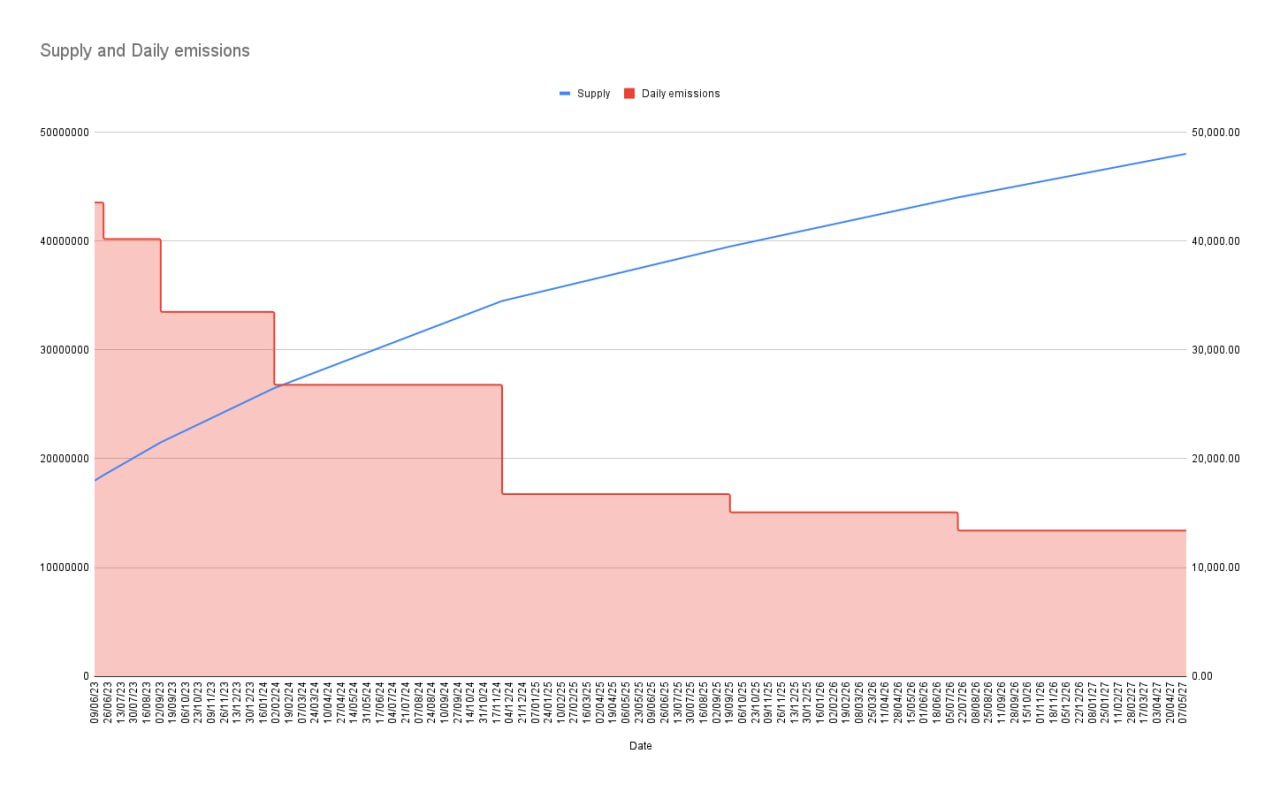
\includegraphics[width=\textwidth]{block_supply}
    \caption{Supply and Daily emissions}
\end{figure}
